\documentclass{ieeeaccess}
\usepackage{cite}
\usepackage{amsmath,amssymb,amsfonts}
\usepackage{algorithmic}
\usepackage{graphicx}
\usepackage{caption}
\usepackage[english]{babel}
\newtheorem{theorem}{Theorem}
\newtheorem{definition}{Definition}
\usepackage{textcomp}
\def\BibTeX{{\rm B\kern-.05em{\sc i\kern-.025em b}\kern-.08em
    T\kern-.1667em\lower.7ex\hbox{E}\kern-.125emX}}
\begin{document}
\history{Date of publication xxxx 00, 0000, date of current version xxxx 00, 0000.}
\doi{10.1109/ACCESS.2017.DOI}

\title{Anonymous provision of local services via blockchain}
\author{\uppercase{Stanis\l{}aw Bara{\'n}ski}\authorrefmark{1}}

\address[1]{Department of Electronic, Telecommunication and Informatics, Gdansk University of Technology, Narutowicza 11/12 Gdansk Poland (e-mail: stanislaw.baranski@pg.edu.pl}

\tfootnote{This paragraph of the first footnote will contain support 
information, including sponsor and financial support acknowledgement. For 
example, ``This work was supported in part by the U.S. Department of 
Commerce under Grant BS123456.''}

\markboth{Bara{\'n}ski : 
Anonymous provision of local services via blockchain}
{Bara{\'n}ski : 
Anonymous provision of local services via blockchain}

\corresp{Corresponding author: Stanislaw Baranski (e-mail: stanislaw.baranski@pg.edu.pl).}

\begin{abstract}
Service providers like lawyers, laboratories, auditors, or banks, to
provide services, require customers to submit data often
associated with their personal information. This situation exposes
customers to privacy risks. However, most service providers use personal information merely for logistic operations like payments
and communication and could provide services anonymously if other means of logistics exist.

We propose a framework for coordinating local anonymous service
provision. Our proposal uses blockchain for both anonymous payments and proofs of existence (so-called message board) and content-addressable network (e.g.~IPFS) for results delivery.

A local service provider can employ our framework to provide
services without collecting any personal information. Possible
applications for this framework include anonymous clinical drug testing,
steroid testing, parenting testing, anonymous legal advice, or
anonymous financial trustworthiness evaluation.

In case of dispute, either due to exceeding deadlines or providing
incorrect results, the customer can disclose the whole interaction and
prove to justice (police or court) the misbehaviour of the service
provider.

We analyse the protocol in the context of fairness and discuss further
extensions to an anonymous delivery system, payment with cash, and
decentralised conflict resolution system.

Our framework can enable various services currently based on unacceptable trust assumptions to the SP.
\end{abstract}

\begin{keywords}
Blockchain, anonymity, fair-exchange, physical delivery
\end{keywords}

\titlepgskip=-15pt

\maketitle
\section{Introduction}
Service providers (SP) like lawyers, laboratories, auditors, or banks,
to provide services, require data that is often associated with the user
identity.

Providing personal information exposes users to privacy risks,
i.e. potential loss of control over personal
information~\cite{smith2011information}.

Such user information can be used deliberately or unintentionally
(e.g., by theft) for insider disclosure, unauthorised access, or
commercial gains. For example, by reselling it to marketers, financial institutions, other businesses, government agencies, or even cybercriminals. Which in turn can lead to profiled advertisements or criminal activities like identity theft or illegal tracking and surveillance~\cite{smith2011information}.

Important individuals like top government, influencers, or celebrities are especially vulnerable to this kind of attack as exposure of their health records, purchase habits, or legal documents can threaten their reputation, position, or can be used for blackmailing.

The guarantee of the privacy of the data is often based merely on a trust assumptions and security of IT system. However, most of the SP do not need the personal information for any other reason than payment or communication, which should be considered secondary compared to actual service provision.

It would be desirable for the user to keep its identity private while the service provider still provides its services. This could lead to reduced trust that users have to put on SP and less responsibility borne by SP.

Example services that would benefit from anonymous services are:
\begin{itemize}
    \item Patients willing to take a steroid test, drug tests, venereal diseases
test, paternity test — have strong incentive to keep the whole
procedure private. Merely the fact that they took the test — without
exposing the results — is suggestive enough to act as a premise in
case of a conflict.

Especially celebrities, politicians and public figures are prone to this kind of problem as such precedent can negatively influence their future career.

Currently, they have to risk that their personal details, materials, and results are stored securely and kept in private from any unauthorised actor (both curious employee, and malicious attacker).

Our protocol allows taking such tests anonymously and therefore getting
rid of the strong trust assumption put on the laboratories and their IT
systems.
\item People willing to take business action that may be risky or not yet fully legislated, may be willing to receive the risk estimation and prediction of possible repercussions of such action.

By exposing our identity to the lawyer, we trust that he won't use that
information for harmful actions.

Our protocol would allow taking such advices anonymously, and therefore
getting rid of the strong trust assumption put on the lawyers and their IT systems.
\end{itemize}

We propose a framework for anonymously provisioning services that require delivery of physical materials. A service provider employing our framework can provide services without collecting any personal information from customers.

In case of dispute, either due to exceeding deadlines or providing
incorrect results, the customer can disclose the whole interaction and
prove to justice (police or court) the misbehaviour of the service
provider.


To achieve these objectives we use:
\begin{itemize}
    \item Privacy-preserving blockchain, to allow customers anonymously pay for the services.
    \item Message board blockchain, to achieve fairness, i.e., as a mean for proving that certain actions took place at a certain moment of time without the trusted third party.
    \item Content-addressable peer-to-peer storage network, to provide results to the customer. 
    \item Cryptography
    \begin{itemize}
        \item Symmetric encryption: to encrypt and decrypt results published on public networks.
        \item Digital signatures: To achieve authentication and non-repudiation of actions. 
    \end{itemize}
    
\end{itemize}

We observe that the issue of anonymous service provision can be seen as a problem of fair-exchange where parties exchange some informations in a fairly manner, i.e., either both parties obtain the goods being exchanged, or they both obtain nothing.

In our case the customer is exchanging with the SP cryptocurrency and materials for the results.

We contribute to the field of fair-exchanges by proposing a simple,
practical, and anonymous framework that does not rely on centralised trusted-third party, but on decentralised blockchain and
distributed content-addressable storage network.

Also, we support physical materials delivery, which was rarely targeted by other researchers or based on strong and unpractical assumptions.

Our framework simultaneously provides five main properties:

\begin{itemize}
\item Anonimity:
throughout the whole transaction the customer stays anonymous to all external observers.
\item Fairness:
at each step of the protocol, both parties are incentivised to act accordingly to the protocol; otherwise the misbehaving party ends up in worst position.
\item Dispute resolution: at each step of the protocol the customer can open a dispute win the case iff the SP misbehaved.
\item TTP-less: 
our protocol does not rely on trusted-third party to conduct transactions in fairly manner. Only in case of dispute the centralised justice is invlolved (the justice decentralisation is discussed in section ~\ref{future-work}.
\item Physical materials: our protocol allows providing not only digital but also physical materials to the service provider.
\end{itemize}

Some authors have proposed blockchain-based fair-exchange systems that could be adapted to service provision; however, to our best knowledge we
are the first to propose a system that satisfy all five properties
stated above. Especially anonimity and physical materials delivery, are
properties that were rarely addressed together, and if so, the protocol
based on TTP, and strong and impractial assumptions on banking system~\cite{birjoveanu2015anonymity}, or didn't address the of conflict
between parties~\cite{altawy2017lelantos}.

Our framework can potentially enable variety of services that for many
customers base on unacceptable trust assumptions to the SP.


\section{State of the art}\label{state-of-the-art}

\paragraph{Anonymity and Fair-Exchange in e-Commerce Protocol for
Physical Products
Delivery}\label{anonymity-and-fair-exchange-in-e-commerce-protocol-for-physical-products-delivery}

Authors of~\cite{birjoveanu2015anonymity} proposed a
fair-exchange of physical product and electronic payment protocol that
guarantee both customer and merchant anonymity. They achieve it by
introducing online trusted third party that validate coins and provide
fair exchange guarantees.

The anonymity is ensured by assuming the existence of source cabinet
(SC) and delivery cabinet (DC), and a trusted delivery agent who take
product from a source cabinet and provide it to a destination cabinet.
Both cabinets provides access to the product by passwords to conceal
identity of the customer and the merchant. To avoid identity disclosure
of customer and merchant, the access to the product is provided by
passwords.

The protocol works as follows: \begingroup
\renewcommand{\labelenumii}{\arabic{enumii}.}

\begin{enumerate}
    \item Both parties agree on the purchase details.
    \item The customer buys a digital coin from his bank and validates it with the TTP.
    \item The customer sends to the merchant the purchase order and the digital signature made by TTP on the encrypted coin.
    \item The merchant post the product to the source cabinet.
    \item Delivery agent collect the product from source cabinet and post it to delivery cabinet.
    \item Customer collects the product from delivery cabinet using password.
    \item The customer checks if the product is actually the ordered one.
    \begin{itemize}
    \item[-] if yes 
        \begin{enumerate}
        \setcounter{enumii}{7}
        \item the customer sends the acknowledge to delivery cabinet and decryption key to the merchant.
        \item The merchant redeem the coins from the bank.
        \end{enumerate}
    \item[-] if no
        \begin{enumerate}
        \setcounter{enumii}{7}
        \item the delivery cabinet is equipment with video camera that records the moment when the customer open the package and let the customer to signal the invalidity of the product, and so, sending the encrypted recording to the TTP. 
        \item the dispute is settled via TTP, optionally letting each party to reveal it's identity.
    \end{enumerate}
    \end{itemize}
\end{enumerate}
\endgroup

Yet, the fair-exchange properties are achieved by strong assumptions.
Namely,

\begin{itemize}
    \item the TTP does not misbehave or collude with any party. 
    \item The customer's and merchant's banks enable confidental transactions and both share commit-buffer where the value is locked until the transaction is finished.   
    \item All banks mantain a global list of coin's serial numbers to prevent double-spending problem. 
    \item The source cabinet and delivery cabinet exists, and in both the product access is protected by password.
    \item Delivery cabinet is equipped with a video camera that records the moment when the customer opens the package, and provide a way to submit the video to TTP in case of a dispute. 
    \item There exists a trusted delivery agent.
    \item Communication channels between parties provides anonymity.
\end{itemize}

\paragraph{Themis: Towards decentralized escrow of cryptocurrencies
without trusted third
parties}\label{themis-towards-decentralized-escrow-of-cryptocurrencies-without-trusted-third-parties}

Themis~\cite{meng2019themis} is a fair-exchange
protocol, which uses blockchain instead of TTP. It provide escrow
services for secure exchanging between cryptocurrencies and digital goods, and decentralised dispute resolution system for resolving conflicts.

Two parties, say Alice and Bob, can create an escrow by generating
2-of-2 (not 2-of-3 as it is other TTP-based systems) threshold account
using Thresh-Key-Gen protocol. Alice and Bob generate secret keys
\(x_A\) and \(x_B\) accordingly, the shared account public key becomes
\(y = g^{x_A+x_B}\); only the access to both Alice's and Bob's secrets
grants access to the shared account.

Then, both Alice and Bob, takes their keys, and split them into
\(n=2t+1\) secret shares using Shamir Secret Shamir protocol, where
\(n\) is the number of mediators that participate in the decentralised
network, and \(t+1\) becomes the threshold of sufficient number of
mediators that can reconstruct the secret key.

Next, both Alice and Bob, take their key shares, and encrypt each
\textit{i}-th key share using public key of \textit{i}-th mediator. As a result
Alice's secret \(x_A\) becomes \({c^A_1, c^A_2,...,c^A_n}\), and Bob's
secret \(x_B\) becomes \({c^B_1, c^B_2,...,c^B_n}\), where
\(c_i = E_{M_i}(P_i)\) is the encrypted \(i\)-th key share using
\(i\)-th mediator public key \(M_i\).

Next, both Alice and Bob exchange the sets of encrypted key shares with
each other, and send funds to the escrow account.

The escrow is secure as long as \(t+1\) of mediators does not collude,
which would let them recreate both \(x_A\) and \(x_B\). Also, to ensure
that parties are exchanging real key shares, they also send a witnesses
generated with Feldman VSS scheme and zero-knowledge proofs to guarantee
the consistency between witnesses and key shares.

In case of dispute, the decentralised network of mediators settle the
conflict and grand one winning party, the other party secret key,
letting him to withdraw the funds.

The honesty of mediators is achieved by the monetary incentivisation and
reputation system.


\paragraph{Lelantos: A blockchain-based anonymous physical delivery
system}\label{lelantos-a-blockchain-based-anonymous-physical-delivery-system}

Lelanros~\cite{altawy2017lelantos} is a blockchain-based anonymous
physical delivery system. The anonymity is achieved by employing ToR's
onion routing to connect physical delivery providers. The whole route
from merchant to customer is split into multiple steps, and each step is
undertaken by different randomly selected delivery provider. As long as
the develiery providers does no collude, mechant can not learn both
identity and destination address of the customer.

Onchain smart-contract is used to coordinate the whole process and
mediate communication between customer and delivery providers.

However, since the system uses Ethereum— fully traceable blockchain—its anonymity is achieved as long as the addresses are not identified with the real identities, which we call pseudonymity rather than anonymity (see section~\ref{pseudo-anon}). Also, the protocol does not cover the case of dispute between the parties.

\section{Background}
\subsection{Dispute resolution system}

Disputes are inevitable part of all human transactions. Whether intentional or accidental, the system should prevent any behaviour volatiling rules of agreed contract or local jurisdiction. The rules are specified by law, and implemented by police.

The vision of smart contract was to replace legal contract with
programmable and autonomous contracts. The specifications of contract
was encompasses in the code, hence the slogan ``code as a law''. Yet,
the blockchain paradigm has its limitations. It can assure the
correctness of data existing on the blockchain. The problem arises on
the contact between blockchain and real world. When we want the smart
contract to make a decision based on some input from outside the
blockchain. We move a lot of trust assumptions on the data providers.
The technique of providing real world data to the blockchain is called
oracle. Oracle provide data based on decentralised network of mediators,
therefore the trust is also decentralised.

Some oracles provide the data like weather, soccer match result, stock
price, train delay, election results, others---and they are the ones we
are interested in---provide the settlement of a submited dispute.


Themis~\cite{meng2019themis} besides providing fair-exchange protocol,
also offers a semi-autonomous decentralised dispute resolution system,
which comply with the web3 postulates of decentralised web. Themis
resolve disputes by set of voluntary anonymous mediators participating
in a voting and deciding whether a party misbehaved. The honesty of
mediators is achieved by the monetary incentivisation and reputation
system.

Kleros~\cite{lesaege2018kleros} is a smart contract deployed on
Ethereum platform that mimics in decentralised and autonomous way how
court works in real life. In Kleros, every process of a dispute like
gathering evidences, selecting jurors, rewarding the winning party is if
automated by a set of smart contracts. Simillar to Themis, the honesty
of the agents voting in a case is achieved by game-theoretical economic
incentives.

Such decentralised, voluntary, and anonymous dispute resolution system
might work for simple contracts violation like eBay seller sending
broken or wrong product, or Airbnb apartment being not adequate to the
photos in the offer. However it's hard to realise such decentralised
evaluation of quality of heath or legal services when expertise and
privacy concerns are taken into an account. Therefore, in our protocol
we take the more conservative approach and resolve disputes using local
justice system (police, court, etc.).

Possible directions toward semi-autonomous decentralised resolution
system are discussed in section ~\ref{future-work}.


\subsection{Proofs to justice}\label{proof-of-justice}
In case of dispute the customer can proof to the justice (police, court,
etc.) evidences that convinces the justice about the honesty of customer
and misbehaviour of SP. The reason why the SP can not start a dispute is
that the customer is anonymous, and therefore there is no personal
information to start a dispute against. To mitigate this issue the SP is
always in advantaged position, so that he has no reason to start a
dispute. The idea described further in section ~\ref{future-work}.

% Unify with what is writen in fiarness analysis



Abstracting from the services the SP is providing, in case of dispute
the customer should be able to prove that: (i) he delivered to the SP a
complete (according to the SP requirements) package, and the SP
accepted it; (ii) he paid for the transaction.

The first proof called proof-of-delivery (PoD) is a confirmation issued
by the SP to the customer.

\[\mathrm{PoD} = (\mathrm{T}_\mathrm{issue}, \mathrm{T}_\mathrm{pay}, \mathrm{T}_\mathrm{provide}, \mathrm{nonce}, \mathrm{sig}_\mathrm{SP})\]

where:

\begin{itemize}

\item
  \(\mathrm{T}_\mathrm{issue}\) - time at which the PoD is issued.
\item
  \(\mathrm{T}_\mathrm{pay}\) - deadline to pay for the transaction.
\item
  \(\mathrm{T}_\mathrm{provide}\) - deadline to provide the service
  results.
\item
  \(\mathrm{nonce}\) - randomly generated number uniquely identifying
  the transaction.
\item
  \(\mathrm{sig}_\mathrm{SP}\) - the SP's signature guaranteeing
  non-repudiation.
\end{itemize}

also:

\(\mathrm{T}_\mathrm{issue} < \mathrm{T}_\mathrm{pay} < \mathrm{T}_\mathrm{provide}\)

The second proof depend on the cryptocurrency implementation and is
discussed further section~\ref{payment-for-services}.

In case the SP has fulfilled the transaction and provide the results,
but the customer unjustly start a dispute, the SP is secured by the
proof of provision (PoP) he has published on the message board (described in section ~\ref{message-board}.

\[\mathrm{PoP} = (\mathrm{cid}, \mathrm{nonce}, \mathrm{sig}_\mathrm{SP})\]

where:

\begin{itemize}

\item
  \(\mathrm{cid}\) - content identifier as specified in section ~\ref{storage-network}.
\item
  \(\mathrm{nonce}\) - the value uniquely identifying the transaction
  previosuly generated in PoD.
\item
  \(\mathrm{sig}_\mathrm{SP}\) - the SP's signature guaranteeing
  non-repudiation.
\end{itemize}

By publishing the PoP on the blockchain, the SP can not falsify the time
at which the results has been provided, because the block creation time
proves that. Blockchain acts as a global clock that securely timestamps
everything that gets into the block, so the PoP that was included in a
block will be associated with the time when the block has been forged.
Moreover, since the blockchain is public, everyone (including the
justice) can be convinced that the SP indeed provided the results at
that time.

The connection between PoP and the results is made by the content
identifier which uniquely points to the results such that the PoP can
not forge results after the publication.

The content identifier is usually some kind of hash write about ipfs

\subsection{Message Board}\label{message-board}
The proof of provision that we coined for the purpose of this protocol
is generaly called the proof of existence
\cite{proofofexistence, de2016stampery, Chainpoi39}.

The idea behind proof of existence is to certify that some information
has existed at a certain moment of time, in such a way that nobody can
undermine its existence, integrity, and ownership (also called the
nonrepudiation requirement).

We need this functionality for two reasons: 1. Communicate the existence
of the results to the customer to whom the SP have no other
communication medium as the customer stays anonymous. 2. Let the SP to
proof the publication of results within the agreed with customer
deadline. Without such a proof there would be no other means to settle
the conflict between the customer claiming the results have not been
published and the SP claiming the results have been published within the
deadline.

Depending on the context the platform of achieving it is called bulletin
board~\cite{achenbach2015improved} or message board~\cite{hinarejos2019solution} or trusted timestamping~\cite{gipp2015decentralized}. In this work we call it message board.

Such functionallity is the easiest to achieve by the trusted third party
that authoritatively tells what happend and when.

Bitcoin introduced a way of decentralising not only the currency system,
but also other similary working centralised trusted third parties
including the message board.

We let keep the protocol general enough to let the implementator use any
existing technology to provide message board service, with the
assumption that it's decentralised and supports subscribing for the
upcoming proofs from particular address.



\subsection{Anonymity, pseudonomity, and confidentality}\label{pseudo-anonymous-vs-anonymous-blockchain}

Privacy is a concept used in almost all kinds of social sciences like philosophy, psychology, sociology, and legal. The multidisciplinary nature leads to ambigous definitions~\cite{smith2011information}. For the purpose of our work we rely on more concrete definitions, i.e.~confidentality and anonimity.

Confidentality is the ability to hide the details of an action from others. Or we can say, that the system guarantee confidentality if for all observers everything they can say about the action is the fact that it happened and nothing more.

Anonymity is a the ability to hide one identity from others. More precisely, the unability to correlate actions performed within the system with the identity of the user. Or we can say, that the system guarantee anonymity if for all observers the actions are equally likely to be associated with any user of the system. However, anonymity is a spectrum rather than dichotomous classification. One method of quantifying level of anonymity is proposed in \textit{k}-anonymity~\cite{sweeney2002k}. It measure the user's anonymity by the number of other users from whom the user can not be distinguished. Concretely, the user is \textit{k}-anonymous if his actions are equally likely associated with \textit{k}-1 other users. The larger \textit{k}, the higher anonymity.

There are also techniques that can be deployed on non-anonymous blockchains, the so called mixers that literaly gather together users into an \textit{anonymity set}, which then collude together in order to launder the transactions, in such a way that to a observer the likelihood of the sender of each transaction was equiprobable for any user from the anonymity set.

Some systems guarantee pseudonomity rather than anonymity. Pseudonomity, allows uses to hide their real identity behind the pseudonim. Despite the whole system is transparent and allows linking actions to one identity, the system is considered anonymous as long as the link between pseudonym and real identity is secret. This assumption is hard to satisfy in practice, as the KYC (Know You Customer) and AML (Anti Money Laundering) regulations require users to reveal their real identity on most of the cryptocurrencies exchanges. This makes the anonymity of the user dependent on the security of the IT system. Moreover, some correlations can be infered merely by the analysis of transactions \cite{androulaki2013evaluating, ober2013structure}.

The relations between these terms are ilustrated in the figure~\ref{fig:anonymity-diagram}.

\begin{figure}[h!]
\caption{}
\centering
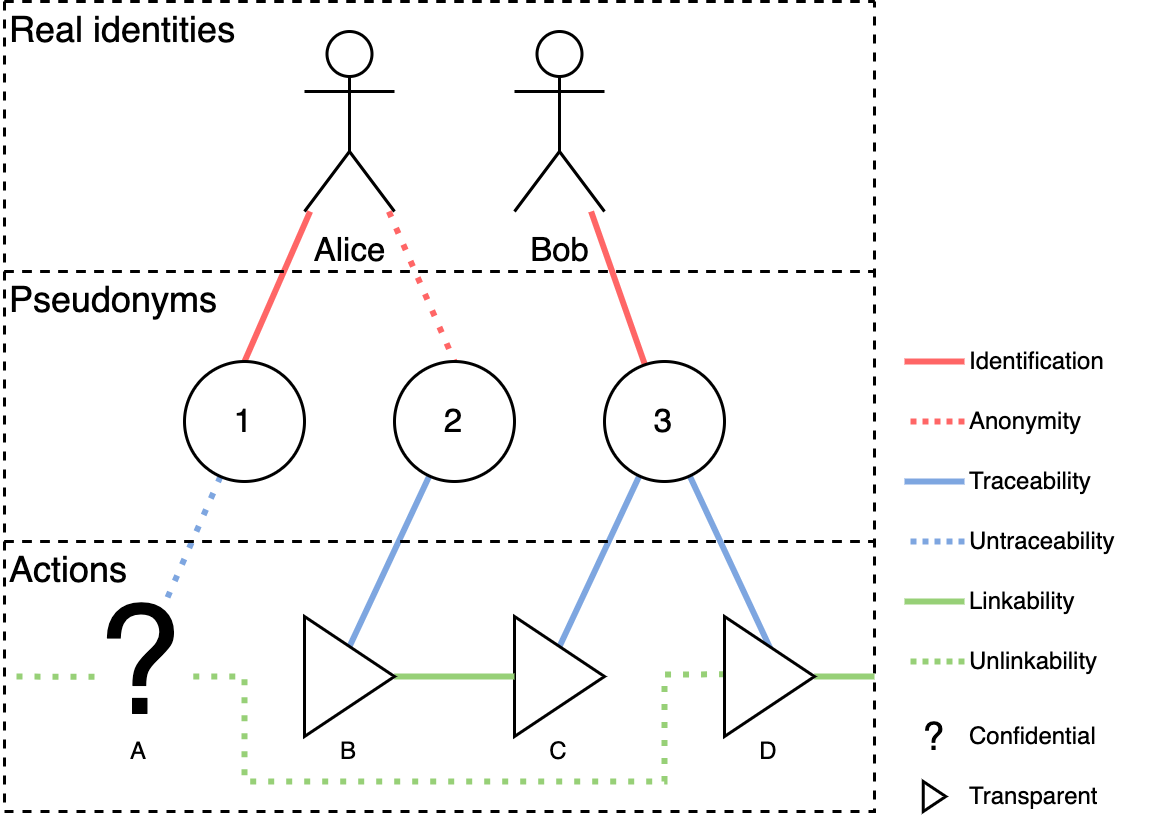
\includegraphics[width=9cm]{anonymity-diagram.png}
\label{fig:anonymity-diagram}
\end{figure}

Let us assume the Alice to be the customer willing to keep her identity private (anonymous) and Bob be the public SP. Alice controls two blockchain addresses 1 and 2, the connection between her real identity and the first address was compromised, and therefore the identification is possible, the connection between the second pseudonym is still unknown therefore anonymous. Alice takes two actions; the first one from the compromised address and the second one from anonymous one. The first action is confidential; therefore even though the psudonym has been compromised the action can not be associated with the Alice. The second action is transparent, therefore the Alice's anonymity is maintained as long as the connection to the second pseudonym is concealed. 

The privacy-preserving blockchains are the ones that maintain anonymity via untraceability and (ideally) unlikability, not via assumption that the connection between an address and the real identity is concealed.   

Blockchains that natively support confidential transactions are
Monero~\cite{van2013cryptonote} (via Ring Signatures~\cite{cryptoeprint:2015:1098} and Bulletproofs~\cite{Bulletpr14, bunz2018bulletproofs}) and ZCash~\cite{sasson2014zerocash} (via zkSNARK~\cite{ben2013snarks}), Grin~\cite{fuchsbauer2019aggregate} (via Mimblewimble~\cite{httpsdow19}).

Overly techniques that achieve anonymity on top of non-privacy-preserving blockchains are: Ethereum's Tornado Cash\cite{pertsev2019tornado} (via zkSNARK~\cite{groth2016size} and MiMC~\cite{albrecht2016mimc}), Bitcoin's Wasabi\cite{WasabiWa56} (via CoinJoin \cite{CoinJoin41}).

\subsection{Payment for services}\label{payment-for-services}
Transactions between customers and SP have to be somehow pegged in order
to prevent proving one payment for multiple transactions. In other
words, we need some way to uniquely link particular payment with the
transaction it pays for.

Depending for the cryptocurrency the link can be created in different
ways:

\begin{itemize}

\item
  separate address — each transaction derives new address uniquely
  associating it with the transaction. Such addresses can be derived
  using Hierarchical Deterministic Wallets (BIP-32)~\cite{bipsbip089}.
\item
  memo — the payments are send to one SP account, but contain extra
  field named ``memo'' which contains a random value generated by SP and
  included in $\mathrm{PoD}$. Each payment containing such value in memo is
  considered to pay for the transaction in question. In case of a dispute,
  the connection can be disclosed by revealing the value in $\mathrm{PoD}$ and payment's memo.
\end{itemize}

Both approaches have some advantages and disadvantages, but our protocol
can abstract them away by treating them as some randomly genrated unique
number, often called \textit{nonce} (number once). How it is implemented
depends on a particular blockchain.

In case of a dispute there must a way to prove to the justice that the
customer has paid for the transaction. As the proof of transaction is
trivial in transparent and trackable blockchains, it gets more
complicated when it comes to anonymous blockchains. Monero allows
proving and checking payments via dedicated API \cite{Howtopro46}.
ZCash provides mechanism called Payment Disclosure \cite{AnIntrod25},
which at the time of writing is still a experimental feature
\cite{paymentd11}.

\subsection{Storage network}\label{storage-network}
Once the SP finish its service, he has to provide the results to the
customer. The most natural approach would to be send the results via
email of decidated platform. However, since the customer wants to stay
anonymous, he don't want to expose his email address nor IP address.
Moreover, in case of dispute the SP should be able to prove that the
results have been provided before the deadline.

One approach would be to post the results into a blockchain. Yet,
storing data on a blockchain is very expensive. The most common
workaround
(\cite{shahid2020blockchain, wang2019auditable, chen2017improved, Usageide95})
is to publish the data to the IPFS \cite{benet2014ipfs}—a content
adressable peer-to-peer storage network—and publish to a blockchain
just a content identifier (cid) that uniquely points to the content
stored on the IPFS.

We take the same approach. Once the SP creates the results, he encrypts
them using the previously provided encryption key; then publish
them into a IPFS network.

To increase anonimity, the customer should use a common techniques to
hide its IP address; for example, use gateway, VPN, proxy, or onion
routing.

\subsection{Separation of concerns}
We could use one blockchain to achieve all of these three roles: (i)
anonymous payments; (ii) message board; (iii) storage network.

As the message board could be achieved by most of the blockchanis, the
anonymous payments isn't so prevalent, and provable storage network is a
functionality of a few specialised blockchains.

Instead of searching for one blockchain that solves all the
functionallities, we allow the framework to use separate blockchains for
each of the functionalities. In case a suitable blockchain arises, it
can play more than one role.

At the time of writing, we see following technologies that fulfill the
requrements of each role:

\begin{enumerate}
\def\labelenumi{\arabic{enumi}.}

\item Anonymous payments: Monero \cite{van2013cryptonote}, ZCash
  \cite{sasson2014zerocash}, Grin \cite{fuchsbauer2019aggregate},
  Tornado Cash \cite{pertsev2019tornado}.
\item Message board: Stampery \cite{de2016stampery}, Proof of Existence
  \cite{proofofexistence} (Bitcoin blockchain), Chainpoint
  \cite{Chainpoi39} (Bitcoin blockchain), or any other blockchain that
  supports attaching extra data along the transaction.
\item Storage network: IPFS \cite{benet2014ipfs}, Filecoin
  \cite{benetfilecoin} (runs on top of IPFS), or Ethereum's
  Swarm\cite{swarmwhi49}.
\end{enumerate}



\section{The Protocol}

\subsection{Prerequisites}
We do not design our framework with the particular technologies in mind, instead we state requirements that each party of the framework must satisfy to make the whole system to work together. The choice of the particular technology for each role is up to the implementer.

\begin{itemize}
\item There exists common PKI infrastructure:
    \begin{itemize}
        \item The customer and the SP have their own key pairs consisting of secret key $\mathrm{sk}(\mathrm{party})$ and public key $\mathrm{pk}(\mathrm{party})$, where $\mathrm{party} \in \{\mathrm{C}, \mathrm{SP}\}$ is the customer or the service provider accordingly.
        \item Both the customer and the SP can create and verify digital signatures created by the customer $\mathrm{sig}_{\mathrm{sk}(\mathrm{C})}$ and the SP $\mathrm{sig}_{\mathrm{sk}(\mathrm{SP})}$.
        \item The SP's public key is publicly known.
    \end{itemize}
    
\item Both the customer and the SP:
    \begin{itemize}
        \item Uses common symmetric encryption $\mathrm{E}_\mathrm{key}(\cdot)$ and decryption $\mathrm{D}_\mathrm{key}(\cdot)$ operations.
    \end{itemize}

\item The SP:
    \begin{itemize}
        \item Accepts packages from unknown customers and give $\mathrm{PoD}$ in return.
        \item Accepts payments with anonymous cryptocurrencies as described in section~\ref{payment-for-services}.
    \end{itemize}
    
\item Justice:
    \begin{itemize}
        \item Accepts as a evidence in dispute a $\mathrm{PoD}$, $\mathrm{PoP}$, and payment $\mathrm{attestation}$ as described in section~\ref{proof-of-justice}.
    \end{itemize}

\item Anonymous payments:
    \begin{itemize}
        \item Supports anonymous, i.e., untraceable and (ideally) unlinkable transactions as specified in section~\ref{pseudo-anonymous-vs-anonymous-blockchain}.
        \item Supports uniquely identifying transaction either via separate address per transaction, memo field, or other similar mechanism as described in section ~\ref{payment-for-services}. 
    \end{itemize}

\item Message board:
    \begin{itemize}
        \item Supports proofs as large as the size of $\mathrm{PoP}$, i.e., sum size of $\mathrm{cid}$, $\mathrm{nonce}$, and $\mathrm{sig}$.
    \end{itemize}

\item The storage network:
    \begin{itemize}
        \item Allows for uniquely content retrieval via $\mathrm{cid}$ (usually a hash of the content).
        \item Allows for anonymous content retrieval.
    \end{itemize}
\end{itemize}

\subsection{Messages}\label{messages}

\paragraph{Package}\label{package}

$$\mathrm{pkg} \equiv (\mathrm{materials}, \mathrm{key})$$

where:

\begin{itemize}

\item $\mathrm{materials}$ - are the materials needed to provide the
  service on. For example, sample of urine, blood, stool, saliva; legal
  documents, CDs, mails, photos, bank statement, or any other kind of
  evidence depending on the service.
\item $\mathrm{key}$ - symmetric key used to encrypt and decrypt the
  results.
\end{itemize}

\paragraph{Proof-of-Delivery}\label{proof-of-delivery}

$$\mathrm{PoD} \equiv (\mathrm{T}_\mathrm{issue}, \mathrm{T}_\mathrm{pay}, \mathrm{T}_\mathrm{provide}, \mathrm{nonce}, \mathrm{sig}_\mathrm{SP})$$

where:

\begin{itemize}

\item $\mathrm{T}_\mathrm{issue}$ - time at which the PoD is issued.
\item
  $\mathrm{T}_\mathrm{pay}$ - deadline to pay for the transaction.
\item
  $\mathrm{T}_\mathrm{provide}$ - deadline to provide the service
  results.
\item $\mathrm{nonce}$ - randomly generated number uniquely identifying
  the transaction.
\item $\mathrm{sig}_\mathrm{SP}$ - the SP's signature guaranteeing
  non-repudiation.
\end{itemize}

also:

\(\mathrm{T}_\mathrm{issue} < \mathrm{T}_\mathrm{pay} < \mathrm{T}_\mathrm{provide}\)

\paragraph{Proof-of-Provision}\label{proof-of-provision}

\[\mathrm{PoP} \equiv (\mathrm{cid}, \mathrm{nonce}, \mathrm{sig}_\mathrm{SP})\]

where:

\begin{itemize}

\item
  \(\mathrm{cid}\) - content identifier as specified in ~\ref{storage-network}.
\item
  \(\mathrm{nonce}\) - the value uniquely identifying the transaction
  previosuly generated in PoD.
\item
  \(\mathrm{sig}_\mathrm{SP}\) - the SP's signature guaranteeing
  non-repudiation.
\end{itemize}

\paragraph{Payment attestation}\label{payment-attestation}

Payment attestation proves that the customer did the payment. Since the
evidences depends on the particular blockchain (see section ~\ref{payment-for-services}). We refer to them symbollicaly as
\(attestation\).

\paragraph{Results}\label{results}

We assume results to be documents in PDF format, but they can be
anything as long as they can be binary encoded and uploaded to IPFS. We
refer to them symbollicaly as \(results\).

\paragraph{Content Identifier (cid)}\label{content-identifier-cid}

Although content identifier (cid) is a term coined by IPFS
\cite{Contenta59}. However, since we our protocol does not depend on
this particular implementation of storage network, we let the cid be any
other identifier that securely and uniquely points to the content.

\subsection{Protocol description}\label{protocol-description}

In this section we describe each step of the protocol. The steps are
shown in the figure ~\ref{fig:protocol-diagram}.

\begin{figure}[h!]
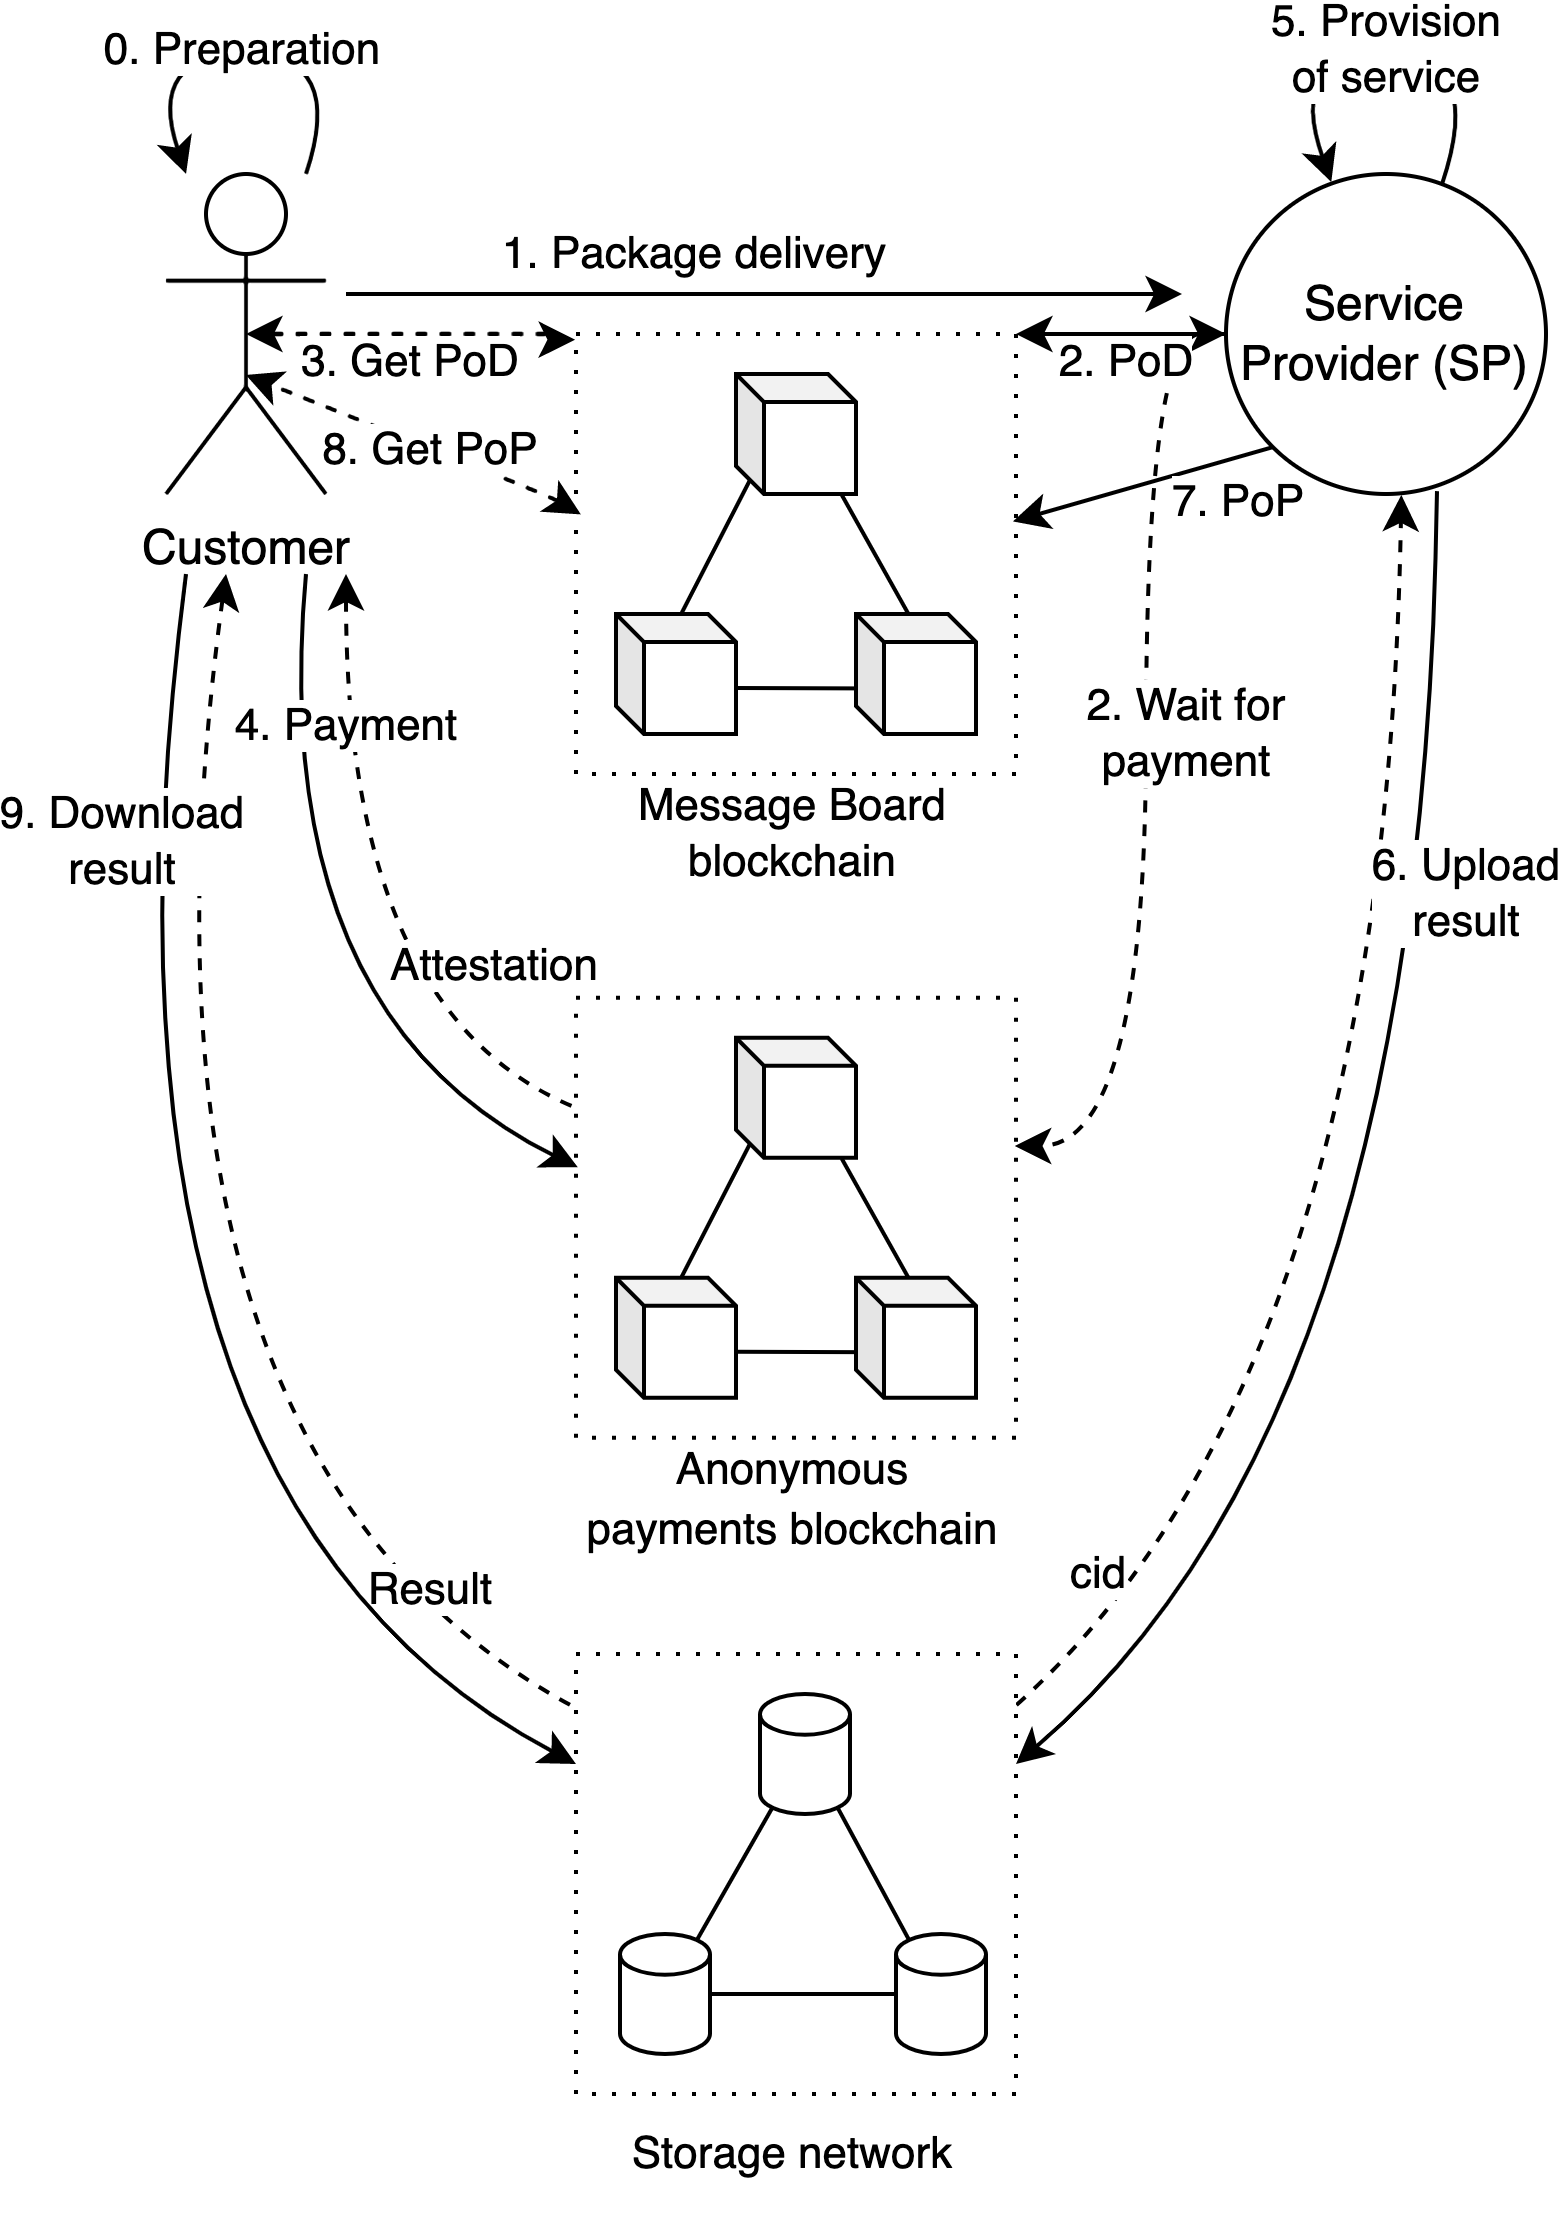
\includegraphics[width=9cm]{anonser-protocol.png}
\centering
\caption{Diagram}
\label{fig:protocol-diagram}
\end{figure}

\paragraph{Step 0: Preparation}\label{step-0-preparation}

The customer collects all the $\mathrm{materials}$ required by the SP, generate an encryption $\mathrm{key}$ print it on a paper as a QR code, and pack them together into a package $\mathrm{pkg}$.

Symbolically: \[
\mathrm{pkg} \gets (\mathrm{materials}, \mathrm{key})
\]

\paragraph{Step 1: Package delivery}\label{step-1-package-delivery}

They protocol starts once the customer delivers package $\mathrm{pkg}$ and the SP accepts its content. In return, the SP issue a $\mathrm{PoD}$ with agreed upfront payment deadline $\mathrm{T}_\mathrm{pay}$, service provision deadline $\mathrm{T}_\mathrm{provide}$ and current time $\mathrm{T}_\mathrm{issue}$. Also, the $\mathrm{PoD}$ consist of randomly generated unique number $\mathrm{nonce}$, which will allow associating all actions related to the transaction throughout the protocol. Finally, the digital signature $\mathrm{sig}_{\mathrm{sk}(\mathrm{SP})}$ on the $\mathrm{PoD}$ created with the SP's secret key $\mathrm{sk}(\mathrm{SP})$ guarantee non-repudiation.

We assume this step to be fully physical, that is, $\mathrm{pkg}$ consist of physical materials, $\mathrm{PoD}$ is in a form of e.g., QR code printed on paper receipt. 

$\mathrm{PoD}$ could be published on a message board (similarly to $\mathrm{PoP}$); however, since the $\mathrm{pkg}$ is delivered personally or via trusted person, the confirmation can be issued in person as well. If we would like to hire a courier to deliver our $\mathrm{pkg}$, then the $\mathrm{PoD}$ would have to be published on message board (further extension to anonymous delivery system is discussed in section \ref{future-work}).

Symbolically: 
\[
\mathrm{PoD} \gets \mathrm{delivery}(\mathrm{pkg})
\]
\[
(\mathrm{T}_\mathrm{issue}, \mathrm{T}_\mathrm{pay}, \mathrm{T}_\mathrm{provide}, \mathrm{nonce}, \mathrm{sig}_{\mathrm{sk}(\mathrm{SP})}) \equiv \mathrm{PoD}
\]


\paragraph{Step 2: Payment}\label{step-2-payment}

Having the PoD issued, the SP can not reject receiving the package. At this point the
customer should pay for the transaction with agreed upfront cryptocurrency system (see section~\ref{payment-for-services}).

In return, the customer receives the $\mathrm{attestation}$ that should be disclosed in case of a dispute.

Symbolically: \[
\mathrm{attestation} \gets \mathrm{payment}(\mathrm{nonce}, \mathrm{sig}_{\mathrm{sk}(\mathrm{C})})
\]

\paragraph{Step 3: Provision of
service}\label{step-3-provision-of-service}
Once the transaction is paid the SP start the provision of service.

Symbolically: \[
\mathrm{results} \gets \mathrm{provision}(\mathrm{materials})
\]

\paragraph{Step 4: Results
upload}\label{step-4-results-upload}

After the service is finished, some kind of output should be created. Next, the output is encrypted using encryption symmetric key $\mathrm{key}$ provided in the first step.

The encrypted results are then uploaded on content addressable network such as IPFS. As a result, the content identifier (cid) is returned.

Symbolically: 
\[
\mathrm{cid} \gets \mathrm{upload}(E_{\mathrm{key}}(\mathrm{results}))
\]

\paragraph{Step 5: Proof of provision
publication}\label{step-5-proof-of-provision-publication}

When the results are published, the SP perform proof of provision by publishing $\mathrm{cid}$ along with $\mathrm{nonce}$ and signature $\mathrm{sig}_\mathrm{SP}$.

Symbolically: 
\[\mathrm{PoP} \equiv (\mathrm{cid}, \mathrm{nonce}, \mathrm{sig}_{\mathrm{sk}(\mathrm{SP})})\]
\[\mathrm{publish}(\mathrm{PoP})\]

\paragraph{Step 6: Proof-of-provision
notification}\label{step-6-proof-of-provision-notification}

After delivering the package and paying for the transaction the customer subscribe to the message board and waits until the SP publish the proof of provision. The subscription is for the SP public key $\mathrm{pk}(\mathrm{SP}$ and transaction's $\mathrm{nonce}$.

Symbolically: \[
\mathrm{cid} \gets \mathrm{subscribe}(\mathrm{pk}(\mathrm{SP}), \mathrm{nonce})
\]

\paragraph{Step 7: Results download}\label{step-7-results-download}
Having the $\mathrm{cid}$, the customer downloads and decrypts the $\mathrm{results}$.

Symbolically: \[
\mathrm{results} \gets \mathrm{D}_{\mathrm{key}}(\mathrm{download}(\mathrm{cid}))
\]


\section{Fairness analysis}
We analyse the fairness of the protocol by representing it as a interactive non-cooperative game.

\subsection{Model}\label{model}
We consider three positions:

\begin{itemize}
\item
  Neutral (•) position: when a party hasn't spend nor gain anything of significant value (money, time, effort). For example, at the beginning of the protocol.
\item
  Disadvantage (-) position: when a party has put a significant value without receiving an equivalent. For example, paid for a service in
  advance.
\item
  Advantage(+) position: when a party would benefit if the transaction would halt at that step. For example, the SP has received payment before service provision.
\end{itemize}

There are many actions that each party can take, but we group them together into two categories:

\begin{enumerate}
\def\labelenumi{\arabic{enumi}.}

\item
  Normal: taking the action prescribed by the protocol.
\item
  Abnormal: everything that deviates from designed steps of the protocol. For example, sending arbitrary message, skipping some step, repeating step, timing out.
\end{enumerate}

Moreover, at any step of the protocol the customer can start a dispute; therefore, another dimension with two positions has to be considered:

\begin{enumerate}
\def\labelenumi{\arabic{enumi}.}

\item
  Agree: the customer agree with the action, and therefore does not start a dispute.
\item
  Start a dispute: the customer does not agree with the action and therefore start a dispute.
\end{enumerate}

As a result, in our analysis we have to consider four different outcomes for each party of the protocol:

\begin{itemize}

\item
  $\sigma_\mathrm{n}$: after following the protocol when the other party acted normally.
\item
  $\sigma_\mathrm{d}$: after a settled dispute when the other party acted normally.
\item
  $\sigma_\overline{n}$: after not starting a dispute despite the other party has acted abnormally.
\item
  $\sigma_\overline{d}$: after a settled dispute when the other party has acted abnormally.
\end{itemize}

The protocol terminate after last step, after starting a dispute, or
after a party hasn't completed it's designated action in time. Therefore,
all positions except $\sigma_\mathrm{n}$ are termination positions.

Because the customer is anonymous the SP can not start a dispute---there is no mean to identify the customer. To mitigate the issue, we designed the protocol so that the SP who follows the protocol is always in advantage position, therefore he has no reason to start a dispute. The customer on the other hand can start a dispute at any time of the protocol, but only the actual misbehaviour of the SP makes him win the case.

\begin{definition}[Fairness] \label{fairness}
A protocol achieve fariness iff 
\begin{equation*}
\begin{split}
\forall_{party \in parties}\forall_{\mathrm{step} \in \mathrm{steps}} &\mathrm{can\ move}\\
&\mathrm{to\ the\ non\ disadvantaged\ position} 
\end{split}
\end{equation*}

\end{definition}


\subsection{Assumptions}\label{assumptions}

For the analysis purpose we state plausable assumptions listed below.

Assumptions:

\begin{itemize}

\item
  Both parties start from neutral position (•).
\item
  Both parties, by completing a transaction, end up in advantaged positions (+). In other words, they have intrinsic motivation to initialise and complete the transaction.
\item
  We assume the steps of the protocol to be atomic, there are no
  intermediate steps.
\item
  Repeating the first step starts new transaction. Repeating any other
  step is considered abnormal and gets ignored. For example paying for
  the invoice twice does not cause any effect on the curse of protocol.
\item
  Once published, the results are available to the customer in the
  content storage. The idea of guaranteeing it cryptographically is
  discussed in section ~\ref{future-work}.
\item
  The protocol can go only forward, there is no way of revert any
  action.
\item
  Losing the dispute leads to punishment that is greater than any
  reward, which leads to disadvantaged position (-). Hence, the rational
  customer won't start a dispute that he is not sure to win.
\item
  Winning the dispute leads to neutral position (•).
\item
  Both the customer and the SP are rational (selfish). They always
  prefer go from worst position to better position, but also risk
  temporary worst position in favour for later better position iff it's
  assured that they won't stuck in worst position.
\end{itemize}

\subsection{Steps}\label{steps}

The table in figure~\ref{fig:positions} shows the positions of each party after each possible
action taken.

\begin{figure}[h!]
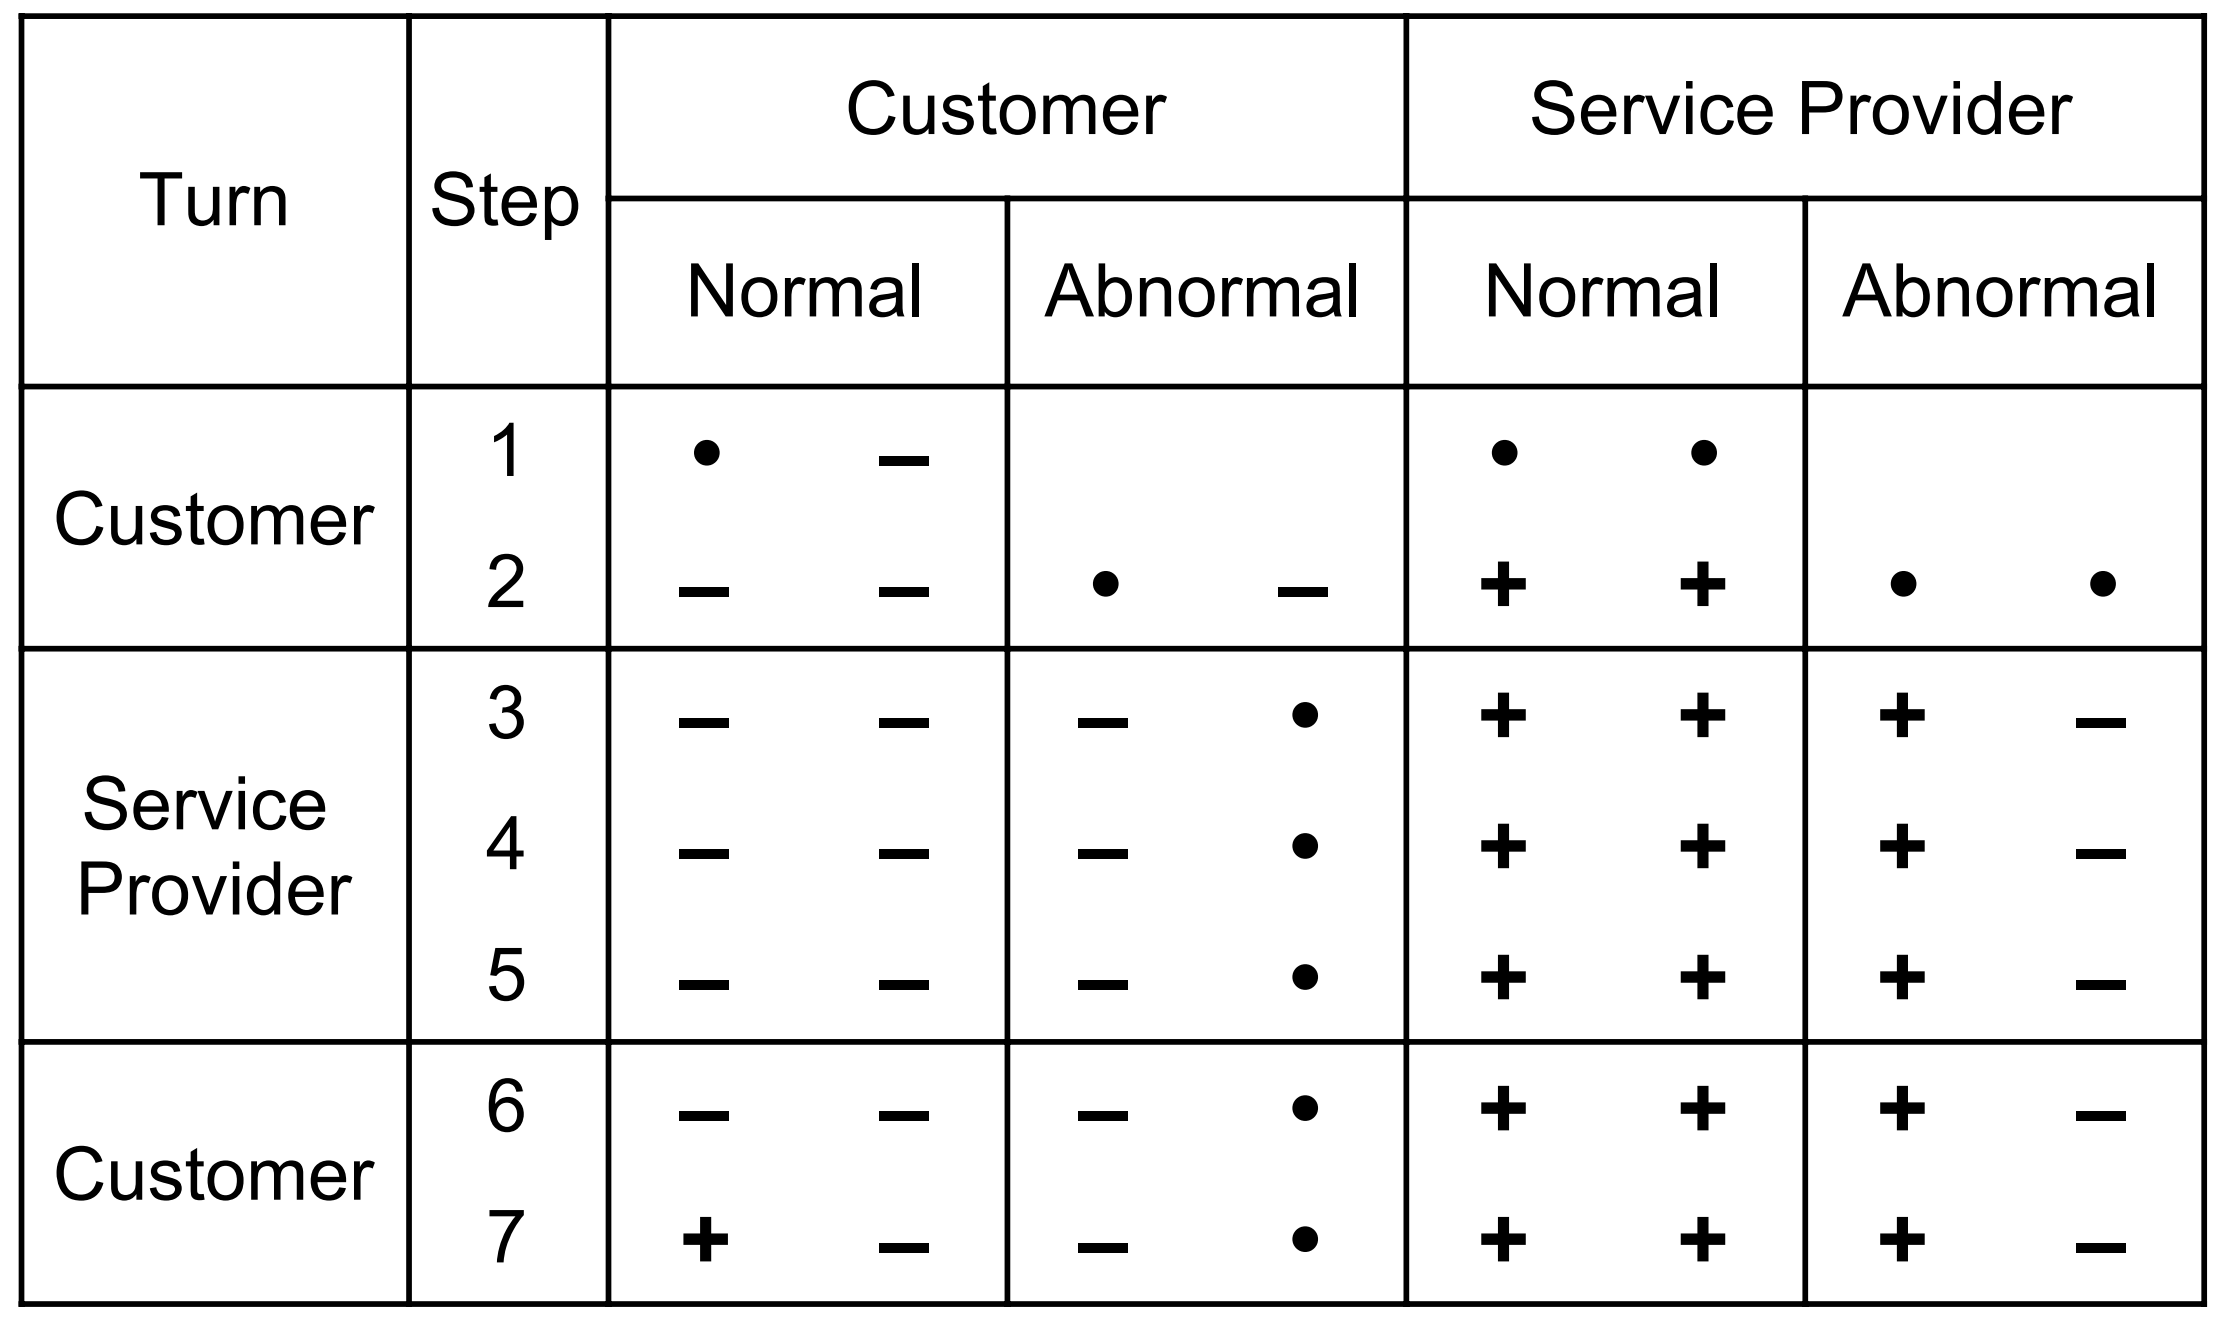
\includegraphics[width=9cm]{formal-table-of-positions.png}
\centering
\caption{Formal table of positions}
\label{fig:positions}
\end{figure}


Below is the description for each step and rationale of the outcome
position.

\paragraph{Step 1, customer turn: deliver package}\label{step-1-deliver-package}

Customer has delivered the package:

\begin{itemize}
\item
  Agreeable path:

  \begin{itemize}
  
  \item
    \(\sigma_{1, c, \mathrm{n}} = •\) - the customer has risked its
    materials but has not paid anything, so we assume he is in neutral
    position (•). One would argue that the customer has put effort of
    delivering the materials to the SP, or that the sample is valuable.
    We assume that the sample without personal information is useless
    and the effort to deliver the package is negligible.
  \item
    \(\sigma_{1, s, \mathrm{n}} = •\) - the SP is in neutral position as
    he didn't put any effort to rece the package, also the package
    hasn't any value to the SP (•).
  \end{itemize}
\item
  Starting a dispute:

  \begin{itemize}
  
  \item
    \(\sigma_{1, c, \mathrm{d}} = -\) - the customer lose the case as
    the SP has still opportunity to publish proof-of-provision within
    timeframe (-).
  \item
    \(\sigma_{1, s, \mathrm{d}} = •\) - the SP win the case for the same
    reason (•).
  \end{itemize}
\end{itemize}

Fairness:

\begin{itemize}

\item
  The customer can follow the protocol and move to the non-disadvantaged
  position \(\sigma_{1, c, \mathrm{n}} = •\).
\item
  The SP can do nothing and end up in non-disadvantaged position
  \(\sigma_{1, s, \mathrm{n}} = •\) or
  \(\sigma_{1, s, \mathrm{d}} = •\).
\end{itemize}

\paragraph{Step 2, customer turn: pay for invoice}\label{step-2-pay-for-invoice}

Customer has paid the invoice:

\begin{itemize}
\item
  Following protocol:

  \begin{itemize}
  
  \item
    \(\sigma_{2, c, \mathrm{n}} = -\) the customer has spend his funds
    but hasn't received the results. Therefore, he moves to the
    disadvantaged position (-).
  \item
    \(\sigma_{2, s, \mathrm{n}} = +\) the SP has received the payment
    but hasn't spend his resources yet. Therefore, he moves to advantaged
    position (+).
  \end{itemize}
\item
  Starting a dispute:

  \begin{itemize}
  
  \item
    \(\sigma_{2, c, \mathrm{d}} = -\) the customer lose the case as the
    SP has still opportunity to publish proof-of-provision before the
    deadline (-)
  \item
    \(\sigma_{2, s, \mathrm{d}} = +\) the SP win the case for the same
    reason (+)
  \end{itemize}
\end{itemize}

Customer has timeouted \(time-to-issue-\), then:

\begin{itemize}
\item
  Following protocol:

  \begin{itemize}
  
  \item
    \(\sigma_{2, c, \overline{\mathrm{n}}} = •\) - the customer ends up
    in neutral position, since he didn't spend his funds (•)
  \item
    \(\sigma_{2, s, \overline{\mathrm{n}}} = •\) - The SP ends up in
    neutral position as he didn't receive the payment, nor spent his
    resources (•)
  \end{itemize}
\item
  Starting a dispute:

  \begin{itemize}
  
  \item
    \(\sigma_{2, c, \overline{\mathrm{d}}} = -\) - the customer loses
    the case as he can not prove the payment before the time limit.
    Consequently, ends up in disadvantaged position (-)
  \item
    \(\sigma_{2, s, \overline{\mathrm{d}}} = •\) - the SP is not charged
    to the justice due to lack of proofs. Therefore, he ends up in
    neutral position (•)
  \end{itemize}
\end{itemize}

Fairness:

\begin{itemize}

\item
  The customer can move the protocol forward to the step 3, where if the
  SP follow the protocol then the customer can push the protocol forward
  up to the last termination step \(\sigma_{7, c, \mathrm{n}} = +\),
  otherwise if at any step the SP does not follow the protocol the
  customer can start a dispute which terminates the protocol at
  non-disadvantaged position, i.e.,
  \(\sigma_{3, c, \overline{\mathrm{d}}} = •\),
  \(\sigma_{4, c, \overline{\mathrm{d}}} = •\),
  \(\sigma_{5, c, \overline{\mathrm{d}}} = •\).
\item
  The SP can do nothing and end up in non-disadvantaged position
  \(\sigma_{2, s, \mathrm{n}} = +\), \(\sigma_{2, s, \mathrm{d}} = +\),
  \(\sigma_{2, s, \overline{\mathrm{n}}} = •\),
  \(\sigma_{2, s, \overline{\mathrm{d}}} = •\).
\end{itemize}

\paragraph{Step 3, SP turn: provision of
service}\label{step-3-provision-of-service}

The SP has done the provision of service:

\begin{itemize}
\item
  Following protocol:

  \begin{itemize}
  
  \item
    \(\sigma_{3, c, \mathrm{n}} = -\) the customer hasn't received the
    results. Therefore, he remains in disadvantaged position (-).
  \item
    \(\sigma_{3, s, \mathrm{n}} = +\) the SP has fullfiled the contract
    on time (+).
  \end{itemize}
\item
  Starting a dispute:

  \begin{itemize}
  
  \item
    \(\sigma_{3, c, \mathrm{d}} = -\) the customer lose the case as the
    SP has still opportunity to publish proof-of-provision within
    timeframe (-)
  \item
    \(\sigma_{3, s, \mathrm{d}} = +\) the SP win the case for the same
    reason (+)
  \end{itemize}
\end{itemize}

SP has timeouted, then:

\begin{itemize}
\item
  Following protocol:

  \begin{itemize}
  
  \item
    \(\sigma_{3, c, \overline{\mathrm{n}}} = -\) the customer ends up in
    disadvantaged position (-)
  \item
    \(\sigma_{3, s, \overline{\mathrm{n}}} = +\) the SP ends up in
    advantaged position as he received the payment (+)
  \end{itemize}
\item
  Starting a dispute:

  \begin{itemize}
  
  \item
    \(\sigma_{3, c, \overline{\mathrm{d}}} = •\) the customer wins the
    case and end up in neutral position (•)
  \item
    \(\sigma_{3, s, \overline{\mathrm{d}}} = -\) the SP loses the case
    and end up in disadvantaged position (-)
  \end{itemize}
\end{itemize}

Fairness:

\begin{itemize}

\item
  The customer can do nothing if the SP follows the protocol, which will
  ultimately put him in advantaged position
  \(\sigma_{7, c, \mathrm{n}} = +\), or in case of the SP not following
  the protocol, the customer can start a dispute and terminate in
  non-disadvantaged position
  \(\sigma_{3, c, \overline{\mathrm{d}}} = •\).
\item
  The SP can follow the protocol and move to the non-disadvantaged
  position \(\sigma_{3, s, \mathrm{n}} = +\), or not follow the protocol
  and also end up at non-disadvantaged position
  \(\sigma_{3, s, \overline{\mathrm{n}}} = +\), but the second option
  puts him at risk of terminating the protocol at
  \(\sigma_{3, s, \overline{\mathrm{n}}} = +\), if the customer is
  rational and starts a dispute.
\end{itemize}

\paragraph{Step 4, SP turn: publication of
results}\label{step-4-publication-of-results}

SP has published results on time:

\begin{itemize}
\item
  Following protocol:

  \begin{itemize}
  
  \item
    \(\sigma_{4, c, \mathrm{n}} = -\) the customer hasn't received the
    results. Therefore, he remains in disadvantaged position (-).
  \item
    \(\sigma_{4, s, \mathrm{n}} = +\) the SP has fullfiled the contract
    on time (+).
  \end{itemize}
\item
  Starting a dispute:

  \begin{itemize}
  
  \item
    \(\sigma_{4, c, \mathrm{d}} = -\) the customer lose the case as the
    SP has still opportunity to publish proof-of-provision within
    timeframe (-)
  \item
    \(\sigma_{4, s, \mathrm{d}} = +\) the SP win the case for the same
    reason (+)
  \end{itemize}
\end{itemize}

SP has timeouted, then:

\begin{itemize}
\item
  Following protocol:

  \begin{itemize}
  
  \item
    \(\sigma_{4, c, \overline{\mathrm{n}}} = -\) the customer ends up in
    disadvantaged position (-)
  \item
    \(\sigma_{4, s, \overline{\mathrm{n}}} = +\) the SP ends up in
    advantaged position as he received the payment (+)
  \end{itemize}
\item
  Starting a dispute:

  \begin{itemize}
  
  \item
    \(\sigma_{4, c, \overline{\mathrm{d}}} = •\) the customer wins the
    case and end up in neutral position (•)
  \item
    \(\sigma_{4, s, \overline{\mathrm{d}}} = -\) the SP loses the case
    and end up in disadvantaged position (-)
  \end{itemize}
\end{itemize}

Fairness:

\begin{itemize}

\item
  The customer can do nothing if the SP follows the protocol, which will
  ultimately put him in advantaged position
  \(\sigma_{7, c, \mathrm{n}} = +\), or in case of the SP not following
  the protocol, the customer can start a dispute and terminate in
  non-disadvantaged position
  \(\sigma_{4, c, \overline{\mathrm{d}}} = •\).
\item
  The SP can follow the protocol and move to the non-disadvantaged
  position \(\sigma_{4, s, \mathrm{n}} = +\), or not follow the protocol
  and also end up at non-disadvantaged position
  \(\sigma_{4, s, \overline{\mathrm{n}}} = +\), but the second option
  puts him at risk of terminating the protocol at
  \(\sigma_{4, s, \overline{\mathrm{n}}} = +\), if the customer is
  rational and starts a dispute.
\end{itemize}

\paragraph{Step 5, SP turn: publication of
proof-of-provision}\label{step-5-publication-of-proof-of-provision}

The SP has published proof of provision on time:

\begin{itemize}
\item
  Following protocol:

  \begin{itemize}
  
  \item
    \(\sigma_{5, c, \mathrm{n}} = -\) the customer hasn't received the
    results. Therefore, he remains in disadvantaged position (-).
  \item
    \(\sigma_{5, s, \mathrm{n}} = +\) the SP has fullfiled the contract
    on time (+).
  \end{itemize}
\item
  Starting a dispute:

  \begin{itemize}
  
  \item
    \(\sigma_{5, c, \mathrm{d}} = -\) the customer lose the case as the
    SP can prove the publication of proof-of-provision (-)
  \item
    \(\sigma_{5, s, \mathrm{d}} = +\) the SP win the case as the SP can
    prove the publication of proof-of-provision (+)
  \end{itemize}
\end{itemize}

SP has timeouted, then:

\begin{itemize}
\item
  Following protocol:

  \begin{itemize}
  
  \item
    \(\sigma_{5, c, \overline{\mathrm{n}}} = -\) the customer ends up in
    disadvantaged position (-)
  \item
    \(\sigma_{5, s, \overline{\mathrm{n}}} = +\) the SP ends up in
    advantaged position as he received the payment (+)
  \end{itemize}
\item
  Starting a dispute:

  \begin{itemize}
  
  \item
    \(\sigma_{5, c, \overline{\mathrm{d}}} = •\) the customer wins the
    case and end up in neutral position (•)
  \item
    \(\sigma_{5, s, \overline{\mathrm{d}}} = -\) the SP loses the case
    and end up in disadvantaged position (-)
  \end{itemize}
\end{itemize}

Fairness:

\begin{itemize}

\item
  The customer can do nothing if the SP follows the protocol, because it
  will ultimately put him in advantaged position
  \(\sigma_{7, c, \mathrm{n}} = +\), otherwise, in case of the SP not
  following the protocol, the customer can start a dispute and terminate
  in non-disadvantaged position
  \(\sigma_{5, c, \overline{\mathrm{d}}} = •\).
\item
  The SP can follow the protocol and move to the non-disadvantaged
  position \(\sigma_{5, s, \mathrm{n}} = +\), or not follow the protocol
  and also end up at non-disadvantaged position
  \(\sigma_{5, s, \overline{\mathrm{n}}} = +\), but the second option
  puts him at risk of terminating the protocol at
  \(\sigma_{5, s, \overline{\mathrm{n}}} = +\), if the customer is
  rational and starts a dispute.
\end{itemize}


\paragraph{Step 6, customer turn: pull
proof-of-provision}\label{step-6-pull-proof-of-provision}

SP has published results on time, then:

\begin{itemize}
\item
  Follows the protocol:

  \begin{itemize}
  
  \item
    \(\sigma_{6, c, \mathrm{n}} = -\) the customer gets hash of the
    results but not the results. Therefore, he is still in disadvantaged
    position(-).
  \item
    \(\sigma_{6, s, \mathrm{n}} = +\) the SP position hasn't changed(+).
  \end{itemize}
\item
  Starts a dispute:

  \begin{itemize}
  
  \item
    \(\sigma_{6, c, \mathrm{d}} = -\) the customer lose the case as the
    SP can prove the publication of proof-of-provision (-)
  \item
    \(\sigma_{6, s, \mathrm{d}} = +\) the SP win the case as the SP can
    prove the publication of proof-of-provision (+)
  \end{itemize}
\end{itemize}

Customer has timeouted, then:

\begin{itemize}
\item
  Follows the protocol:

  \begin{itemize}
  
  \item
    \(\sigma_{6, c, \overline{\mathrm{n}}} = -\) the customer ends up in
    disadvantaged position (-)
  \item
    \(\sigma_{6, s, \overline{\mathrm{n}}} = +\) the SP ends up in
    advantaged position as he received the payment but didn't spend his
    resources (+)
  \end{itemize}
\item
  Starts a dispute:

  \begin{itemize}
  
  \item
    \(\sigma_{6, c, \overline{\mathrm{d}}} = •\) the customer wins the
    case and end up in neutral position (•)
  \item
    \(\sigma_{6, s, \overline{\mathrm{d}}} = -\) the SP loses the case
    and end up in disadvantaged position (-)
  \end{itemize}
\end{itemize}

Fairness:

\begin{itemize}

\item
  The customer can follow the protocol to the position
  \(\sigma_{6, c, \mathrm{n}} = -\), which let's him move the protocol
  to non-disadvantaged termination position
  \(\sigma_{7, c, \mathrm{n}} = +\), or in case the SP haven't followed
  the protocol start a dispute and win the case
  \(\sigma_{6, c, \overline{\mathrm{d}}} = •\).
\item
  The SP can do nothing and end up in non-disadvantaged position
  \(\sigma_{6, s, \mathrm{n}} = +\), or
  \(\sigma_{6, s, \overline{\mathrm{n}}} = +\).
\end{itemize}

\paragraph{Step 7, customer turn: retrieval of
results}\label{step-7-retrieval-of-results}

SP has published \textbf{correct} results on time:

\begin{itemize}
\item
  Following protocol:

  \begin{itemize}
  
  \item
    \(\sigma_{7, c, \mathrm{n}} = +\) the customer gets the correct
    results. Therefore, he moves to advantaged position (+).
  \item
    \(\sigma_{7, s, \mathrm{n}} = +\) the SP position hasn't changed
    (+).
  \end{itemize}
\item
  Starting a dispute:

  \begin{itemize}
  
  \item
    \(\sigma_{7, c, \mathrm{d}} = -\) the customer lose the case as the
    SP can prove the publication of proof-of-provision (-)
  \item
    \(\sigma_{7, s, \mathrm{d}} = +\) the SP win the case as the SP can
    prove the publication of proof-of-provision (+)
  \end{itemize}
\end{itemize}

SP has published \textbf{incorrect} results on time:

\begin{itemize}
\item
  Following protocol:

  \begin{itemize}
  
  \item
    \(\sigma_{7, c, \overline{\mathrm{n}}} = -\) customer end up in
    disadvantaged position, as he ends up with incorrect results (-)
  \item
    \(\sigma_{7, c, \overline{\mathrm{n}}} = +\) SP ends up in advantaged
    position as he received the payment but didn't spend his resources
    (+)
  \end{itemize}
\item
  Starting a dispute:

  \begin{itemize}
  
  \item
    \(\sigma_{7, c, \overline{\mathrm{d}}} = •\) customer wins the case and ends up in neutral position (•)
  \item
    \(\sigma_{7, c, \overline{\mathrm{d}}} = -\) SP lose the case and end up in disadvantaged position (-)
  \end{itemize}
\end{itemize}

Fairness:

\begin{itemize}

\item
  The customer can follow the protocol to the non-disadvantaged termination position \(\sigma_{7, c, \mathrm{n}} = +\), or in case the SP haven't followed the protocol start a dispute and win the case \(\sigma_{7, c, \overline{\mathrm{d}}} = •\).
\item
  The SP can do nothing and end up in non-disadvantaged position \(\sigma_{7, s, \mathrm{n}} = +\).
\end{itemize}

\subsection{Example scenarios}\label{example-scenarios}

The diagram below shows the path of positions when SP try to misbehave and don't execute service after receiving the payment. The protocol ends up in neutral to customer and disadvantaged to SP positions.

\begin{figure}[h!]
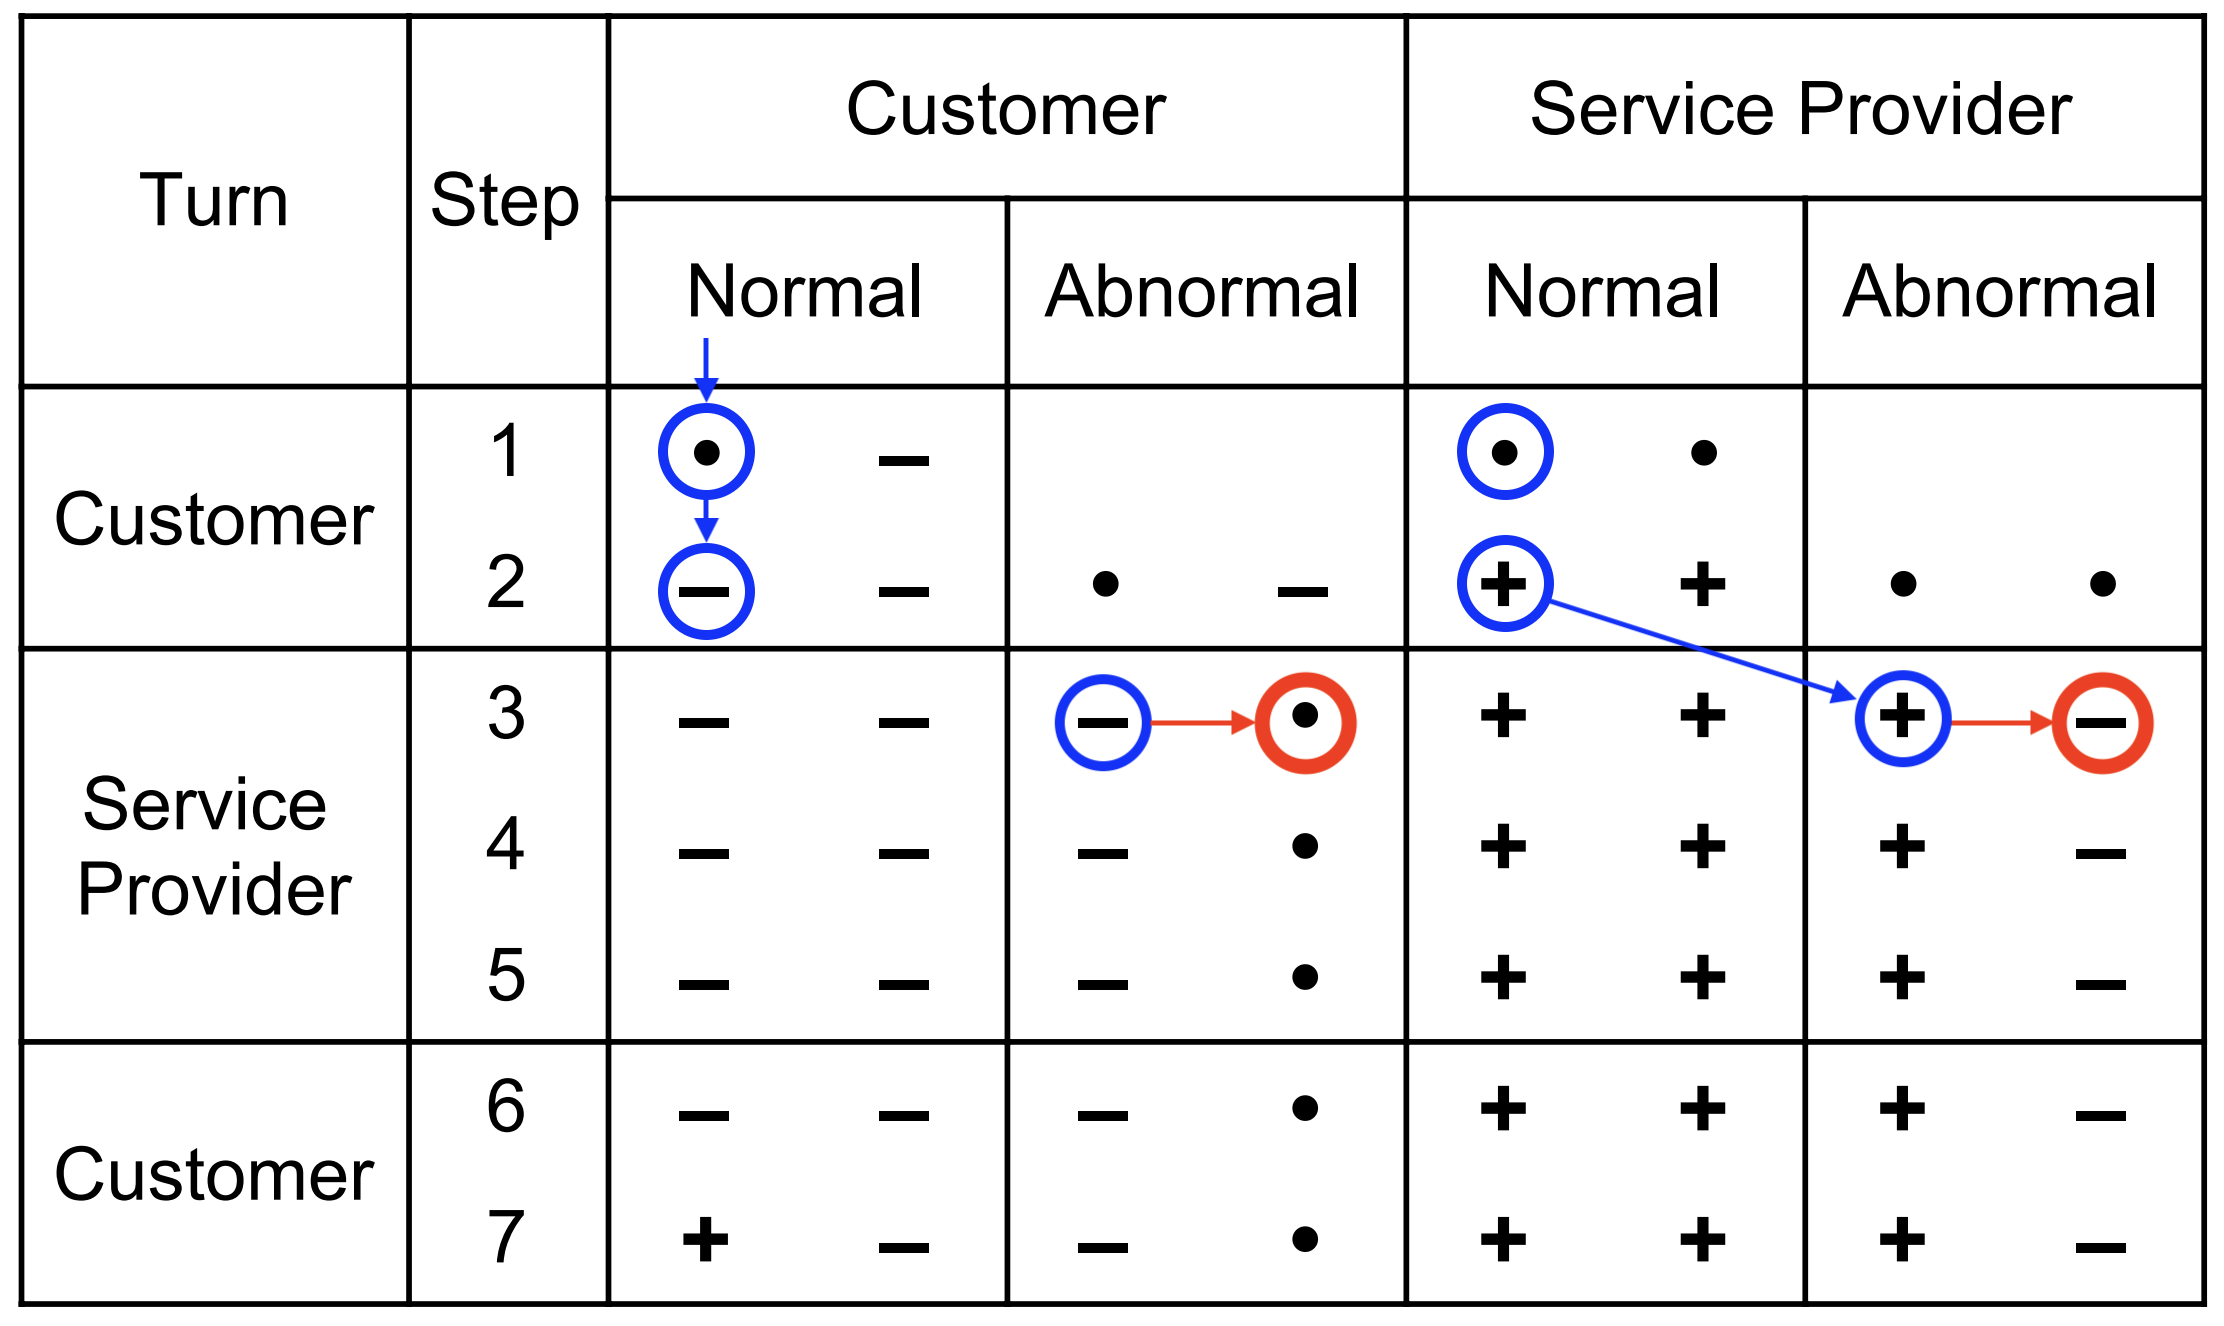
\includegraphics[width=9cm]{formal-misbehaviour-path.png}
\centering
\caption{Scenario of paths where the SP is misbehaving and the customer starts a dispute}
\label{fig:misbehaviour}
\end{figure}

Ultimately, the rational path for both parties is to follow the protocol as shown in the diagram below.

\begin{figure}[h!]
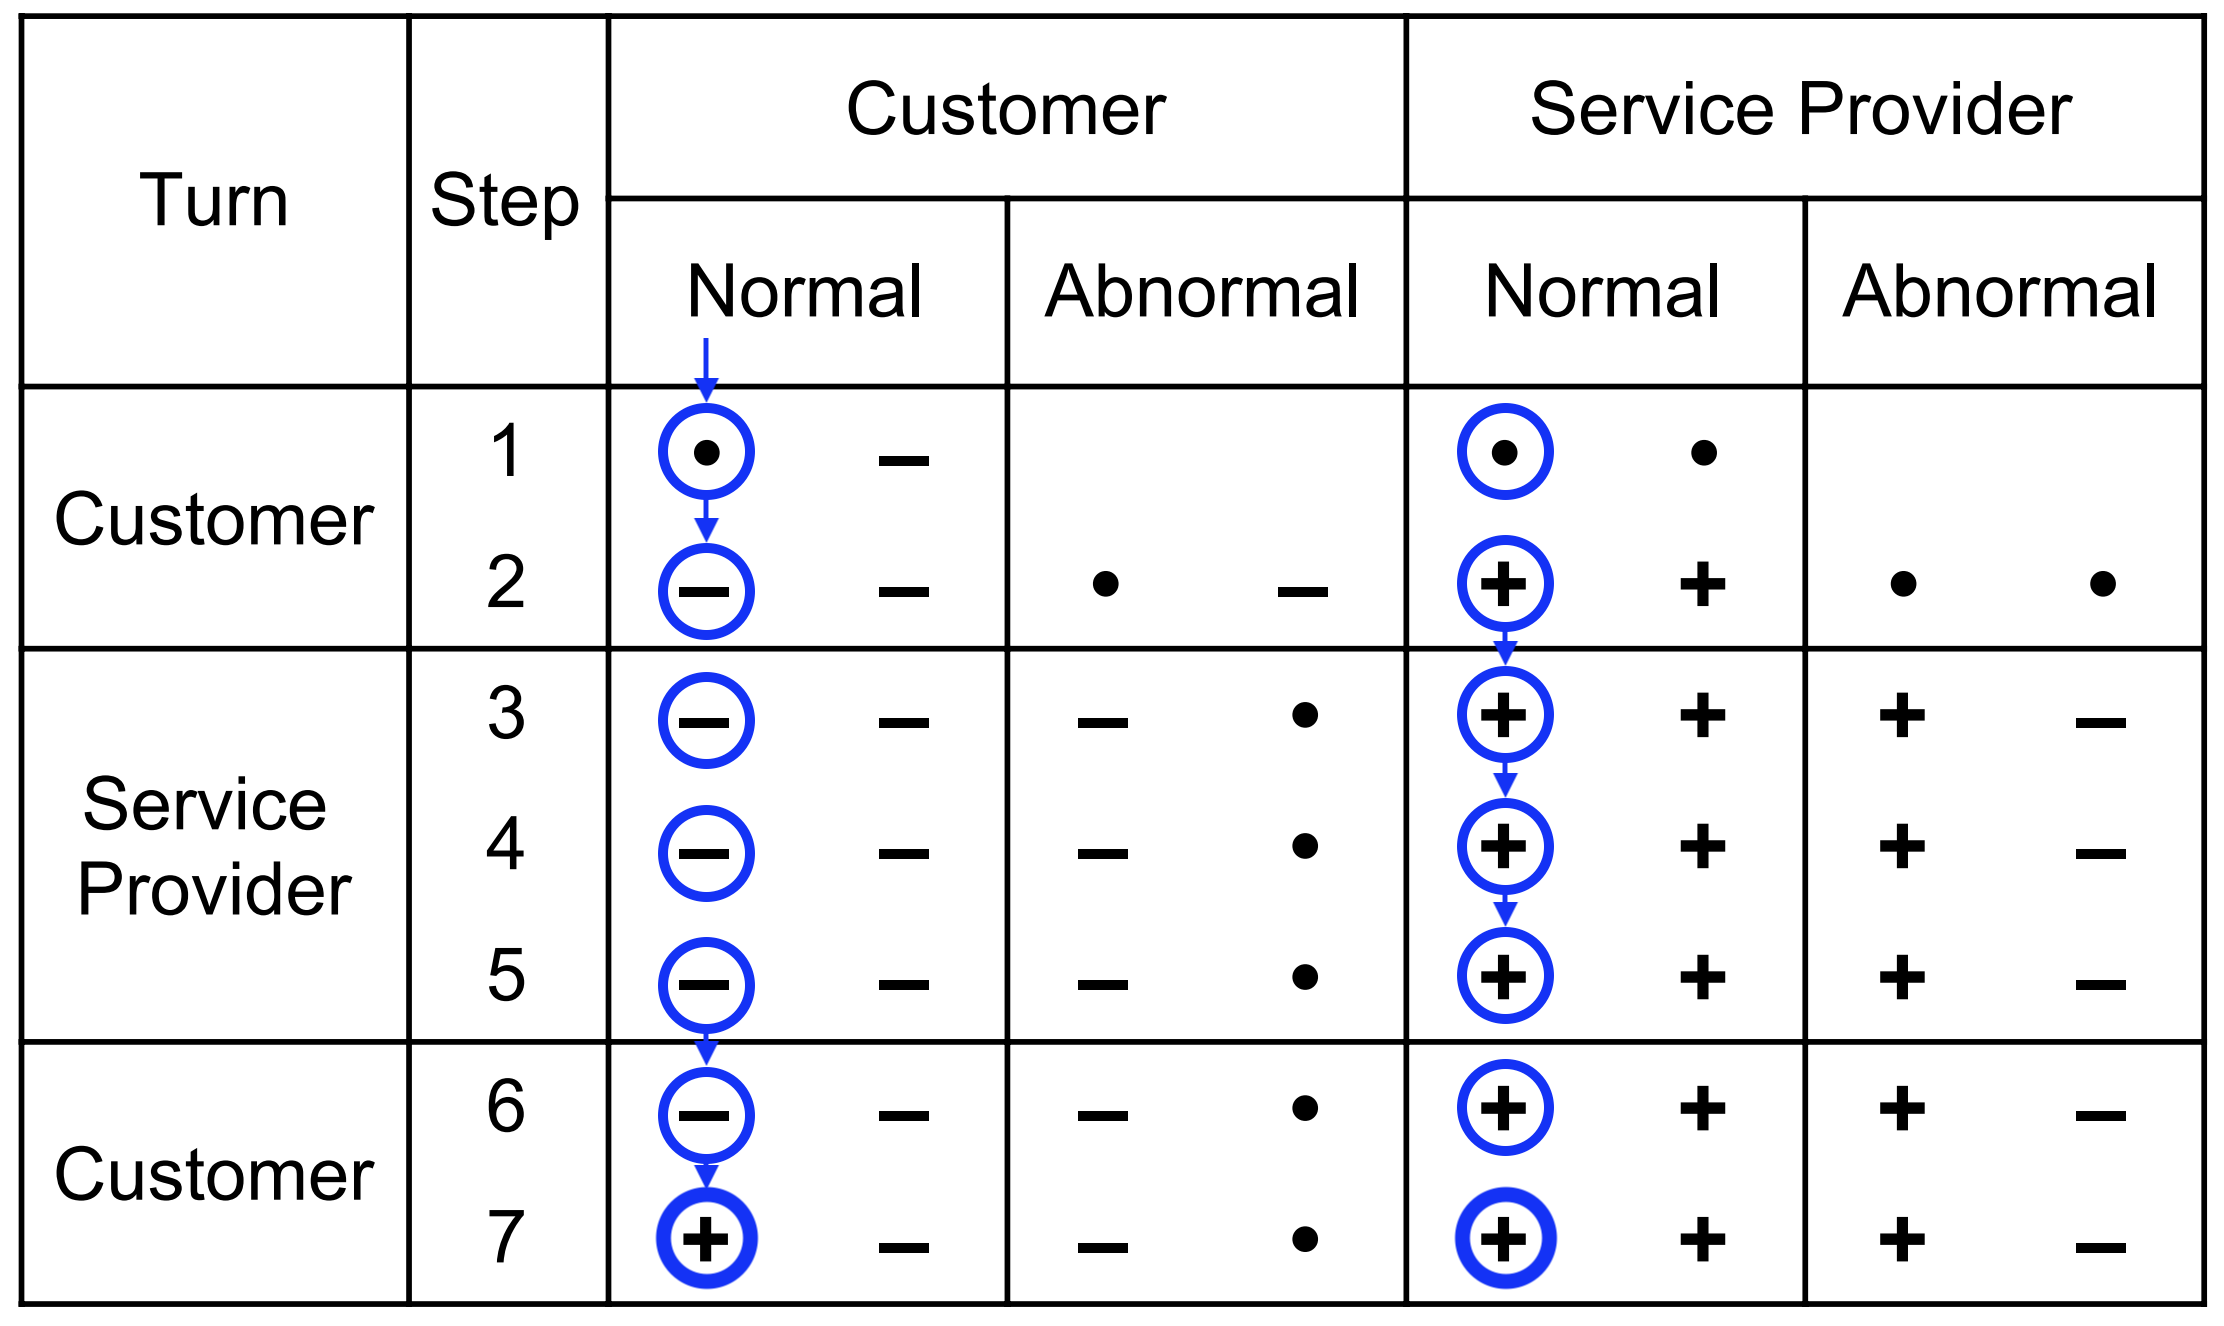
\includegraphics[width=9cm]{formal-rational-path.png}
\centering
\caption{Scenario of path where both the customer and  the SP are behaving correctly}
\label{fig:well-behaviour}
\end{figure}

\subsection{Results}\label{results}

With the fairness definition stated in equation, and the assumptions stated in \ref{assumptions}, our analysis indicate that the protocol achieve fairness.



\section{Future work}\label{future-work}
\subsection{Justice}\label{justice}

Justice is the one biggest obstacle in achieving system that complies with Web3 postulates~\cite{Web3Wiki71}.

The possible directions for mitigation of such issue are to either (1) replace justice with decentralised autonomous organisations (DAO) like proposed in Themis~\cite{meng2019themis} or Kleros~\cite{lesaege2018kleros}; or (2) make it infeasible to provide incorrect results.

The first approach is more feasible in the near future. It would require creating large pool of experts in a field, that in case of dispute, would receive all the proofs (POD, POP, as well as any other proofs significant to the case) that could be queried by the experts in zero-knowledge fashion, i.e., they could ask limited number of questions to the proofs and getting yes/no answers. Keeping the case fully confidential. The experts would be incentivised to participate in the pool by the system of fees. Their honest behaviour would be incentivised by the stake they would have to lock, and punishment they would get by judging incorrectly, where the ``correctly'' is determined by the quorum of votes.

The second approach is more philosophical and visionary. Suppose that the service we are undertaking is fully computable. Then, it would be possible by employing proofs of correctness of computations~\cite{ben2013snarks} to enforce that only correct computations (hence correct services) are accepted. To do so the whole service examination would have to be computable, which is hard to achieve in settings where physical materials (like blood) are examined. Concretely, the problem canes down to ``How to digitally represent blood''. If we could represent urine, blood, saliva, or any other physical material in binary format, and let the customer to take a sample, discrete it and send it to the SP by himself, then the whole chain of integrity could be ensured. Therefore, wrong service provision would be infeasible.


\subsection{Provable availability of
results}\label{cryptographically-provable-availability-of-results}

Currently, the SP has to publish the results into a p2p content addressable storage network, e.g., IPFS. The problem is that, nothing prevent the SP from publishing the results, receiving the cid, publishing $\mathrm{PoP}$, and immediately after removing the results from the local storage. In case of dispute the SP can upload the content again, proving its availability. The SP has no motivation to proceed with this kind of misbehaviour, other than putting the customer in disadvantaged position caused by the lost dispute. We see possible prevention of this misbehaviour by the usage of Filecoin---an incentive layer on top of IPFS that guarantee the content availability via economic incentivisations~\cite{benetfilecoin}. With the help of Filecoin, the SP would be obligated to create a deal that guarantee the results availability until the deadline of the transaction. Moreover, since Filecoin is a blockchain by itself, it could play both roles of message board and storage network.

\subsection{Paying with cash}\label{paying-with-cash}

Without lose of generality the payment can be made with cash. The customer can exchange the cash with SP together with delivering the package. The $\mathrm{PoD}$ would contain an information that the transaction has been paid with cash; therefore, Steps 1 and 2 could be merged together and realised in one step. In case of dispute the payment disclosure would be in included in $\mathrm{PoD}$.

\subsection{Anonymous delivery}\label{anonymous-delivery}

We assumed the customer to deliver the package to the SP personally or via trusted person. However the system could be extended to support anonymous delivery system as proposed in Lelantos~\cite{altawy2017lelantos}.

\section{Conclusions}
In this paper, we have proposed a anonymity- preserving blockchain-based framework for local services provision. The framework can be employed by any local service provider to provide services without collecting any personal information. The payment is handled by anonymous cryptocurrencies. Proof of delivery and proof of provision are published on message board blockchain. The results are published on content addressable p2p network. The dispute can be settled by disclosing proofs to justice. Assuming the definition~\ref{fairness} we showed that the protocol achieve fairness. Finally, we pinpointed further improvements like decentralised dispute resolution, provable  availability of results, paying with cash, and anonymous delivery via courier.

\bibliographystyle{IEEEtran}
% argument is your BibTeX string definitions and bibliography database(s)
\bibliography{bibliography}
\EOD

\end{document}

\setcounter{page}{0}
\newcommand{\floor}[1]{\left\lfloor #1 \right\rfloor}
\newcommand{\ceil}[1]{\left\lceil #1 \right\rceil}
